%%%%%%%%%%%%%%%%%%%%%%%%%%%%%%%%%%%%%%%%%%%%%%%%%%%%%%%%%%%%%%%%%%%%%%%%%%%%%%%%
%2345678901234567890123456789012345678901234567890123456789012345678901234567890
%        1         2         3         4         5         6         7         8

\documentclass[letterpaper, 10 pt, conference]{ieeeconf}  % Comment this line out if you need a4paper

%\documentclass[a4paper, 10pt, conference]{ieeeconf}      % Use this line for a4 paper

\IEEEoverridecommandlockouts                              % This command is only needed if 
                                                          % you want to use the \thanks command

\overrideIEEEmargins                                      % Needed to meet printer requirements.

% See the \addtolength command later in the file to balance the column lengths
% on the last page of the document

% The following packages can be found on http:\\www.ctan.org
\usepackage{graphicx} % for pdf, bitmapped graphics files
%\usepackage{epsfig} % for postscript graphics files
%\usepackage{mathptmx} % assumes new font selection scheme installed
%\usepackage{times} % assumes new font selection scheme installed
\usepackage{amsmath} % assumes amsmath package installed
\usepackage{amssymb}  % assumes amsmath package installed
\usepackage{multicol}

\title{\LARGE \bf
Side Channel Power Analysis of an Embedded Device Running DES  
}


\author{Justin Cox and Tyler Travis
\\ \small{Department of Electrical and Computer Engineering}
\\ \small{Utah State University}
\\ \small{Logan, Utah 84322}
\\ \small{email: justin.n.cox@gmail.com, tyler.travis@aggiemail.usu.edu}
}

\usepackage{listings}
\usepackage{color}

\definecolor{dkgreen}{rgb}{0,0.6,0}
\definecolor{gray}{rgb}{0.5,0.5,0.5}
\definecolor{mauve}{rgb}{0.58,0,0.82}

\lstset{frame=none,
  language=C,
  aboveskip=3mm,
  belowskip=3mm,
  showstringspaces=false,
  columns=flexible,
  basicstyle={\small\ttfamily},
  numbers=none,
  numberstyle=\tiny\color{gray},
  keywordstyle=\color{blue},
  commentstyle=\color{dkgreen},
  stringstyle=\color{mauve},
  breaklines=true,
  breakatwhitespace=true,
  tabsize=3
}

\begin{document}



\maketitle
\thispagestyle{empty}
\pagestyle{empty}


%%%%%%%%%%%%%%%%%%%%%%%%%%%%%%%%%%%%%%%%%%%%%%%%%%%%%%%%%%%%%%%%%%%%%%%%%%%%%%%%
\begin{abstract}

Hardware security is an ever increasing area of study since exploits have been found on computer systems.  Encryption algorithms are very difficult to break.  Instead of breaking the encryption algorithm, it is common for an attacker to attempt to recover the encryption key instead.  One way of recovering the key is using side channel analysis    .  This paper will discuss a side channel analysis performed on a microcontroller that is operating as a crypto device.  The power traces collected will then be analyzed using Differential Power Analysis (DPA) and the results will be shown and discussed.

\emph{Index Terms}---encryption, decryption, security, DPA, side channel.

\end{abstract}

%%%%%%%%%%%%%%%%%%%%%%%%%%%%%%%%%%%%%%%%%%%%%%%%%%%%%%%%%%%%%%%%%%%%%%%%%%%%%%%%
\section{INTRODUCTION}

Through side channel analysis, an attacker is able to leak information   about a device through natural or physical means.  In regards to a device running a crypto algorithm, side channel analysis can be used to leak the encryption key.  There a many different kinds of side channel attacks, but this paper will focus on obtaining information from the power consumed by the target device.  Different operations and data bits require different amounts of power consumption.  By recording and analyzing the power consumption, it is possible to obtain the encryption key.  The encryption algorithm used in this paper is the Data Encryption Standard (DES).

A DES algorithm will be programmed and uploaded onto a TI Tiva C microcontroller.  The algorithm will be ran for many different plaintext inputs and the power consumption will be recorded using an oscilloscope.  The power traces will then be analyzed and it will be determined whether or not the secret encryption key can be obtained.  

%%%%%%%%%%%%%%%%%%%%%%%%%%%%%%%%%%%%%%%%%%%%%%%%%%%%%%%%%%%%%%%%%%%%%%%%%%%%%%%%
\section{DES}

\subsection{Overview and Implementation}

The type of encryption programmed on the microcontroller will be DES.  Although DES is not the current encryption standard and is not as secure as the Advanced Encryption Standard AES, DES is still used in devices today and side channel analysis of a DES crypto device is a valid security risk.

A brief overview of DES will be given so that the reader has a better understanding of how the algorithm works and will better understand where DPA can be used.  If the reader would like an in-depth understanding of DES, it is recommended that the reader look to other sources.

The DES algorithm takes a 64-bit plaintext input.  It is then run through an initial permutation that outputs 56-bits which are then split into two halves.  The data goes through sixteen rounds that each have a sub-key that is generated for each round based on the original 64-bit DES key.  After the sixteenth round, the output is run through a finial permutation and the algorithm outputs a 64-bit encrypted ciphertext.  The rounds are illustrated in Figure 1.

\begin{figure}[thpb]
	\centering
	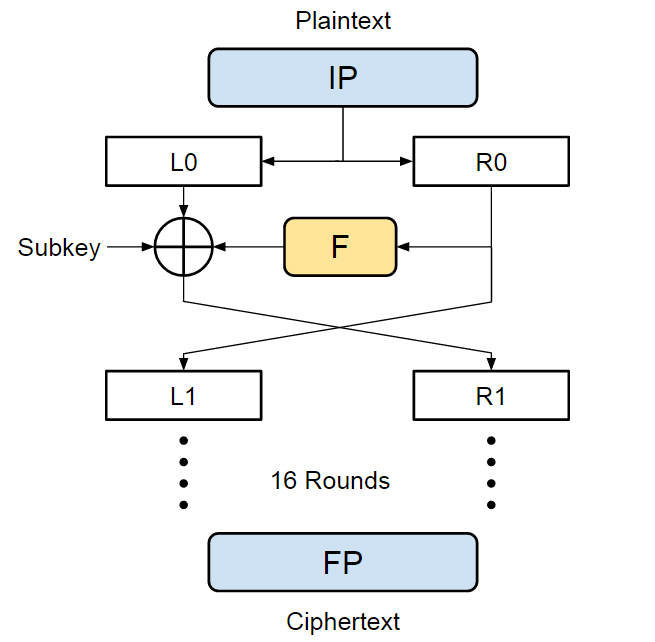
\includegraphics[scale=.50]{DesRounds}
    \caption{An illustration of the sixteen round DES algorithm.}
\end{figure}

During each round, the left 32-bit halve is XORed with the sub key corresponding to the current round as well as the output of the F-function.  The inside functionality of the F-function is illustrated in Figure 2. The output of the XOR is used as the next round's right halve and the next round's left halve is the previous round's right halve.

\begin{figure}[thpb]
	\centering
	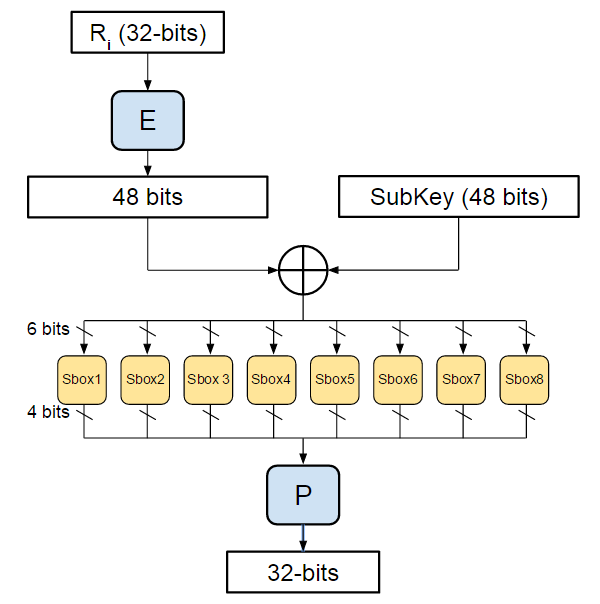
\includegraphics[scale=.50]{Ffunction}
    \caption{An illustration of the F-function.}
\end{figure}

\subsection{Modifications}

There were a few minor changes made to the DES algorithm to facilitate the capturing of power traces.  These changes do not decrease the security of the DES algorithm.  The following assembly routine was added during the last round of the DES algorithm: 

\begin{lstlisting}
	MOVS		r2,#0x00	;Set r2 = 0 
	LDR     	r5,[pc,#1012]	;Lower GPIO PIN  
	LDR		r5,[r5,#0x00]
	BIC     	r5,r5,#0x10
	LDR     	r6,[pc,#1008]  
	STR     	r5,[r6,#0x3FC]
 
 	NOP           
   NOP
   NOP           
   NOP                             
    
   EOR      r2,r4,r3	;<--Instruction of Interest
 
	LDR 		r5,[pc,#992]	;Set GPIO Pin High  
	LDR    	r5,[r5,#0x3FC]
	ORR    	r5,r5,#0x10
	LDR     	r6,[pc,#984]  
	STR     	r5,[r6,#0x3FC]
	
	NOP           
   NOP
   NOP           
   NOP
	
\end{lstlisting}

\noindent
A GPIO pin on the microcontroller is transitioned from a high to a low in order to trigger the oscilloscope to capture the XOR operation that works with the bits of interest for the DPA.  The register that holds the value of the XOR is explicitly set to 0x00 in order to make it easier to measure the Hamming Weight and Distance of that register.  This information is helpful for a Correlation Power Analysis (CPA).

%%%%%%%%%%%%%%%%%%%%%%%%%%%%%%%%%%%%%%%%%%%%%%%%%%%%%%%%%%%%%%%%%%%%%%%%%%%%%%%%
\section{EXPERIMENTAL SETUP}

\begin{figure}[thpb]
	\centering
	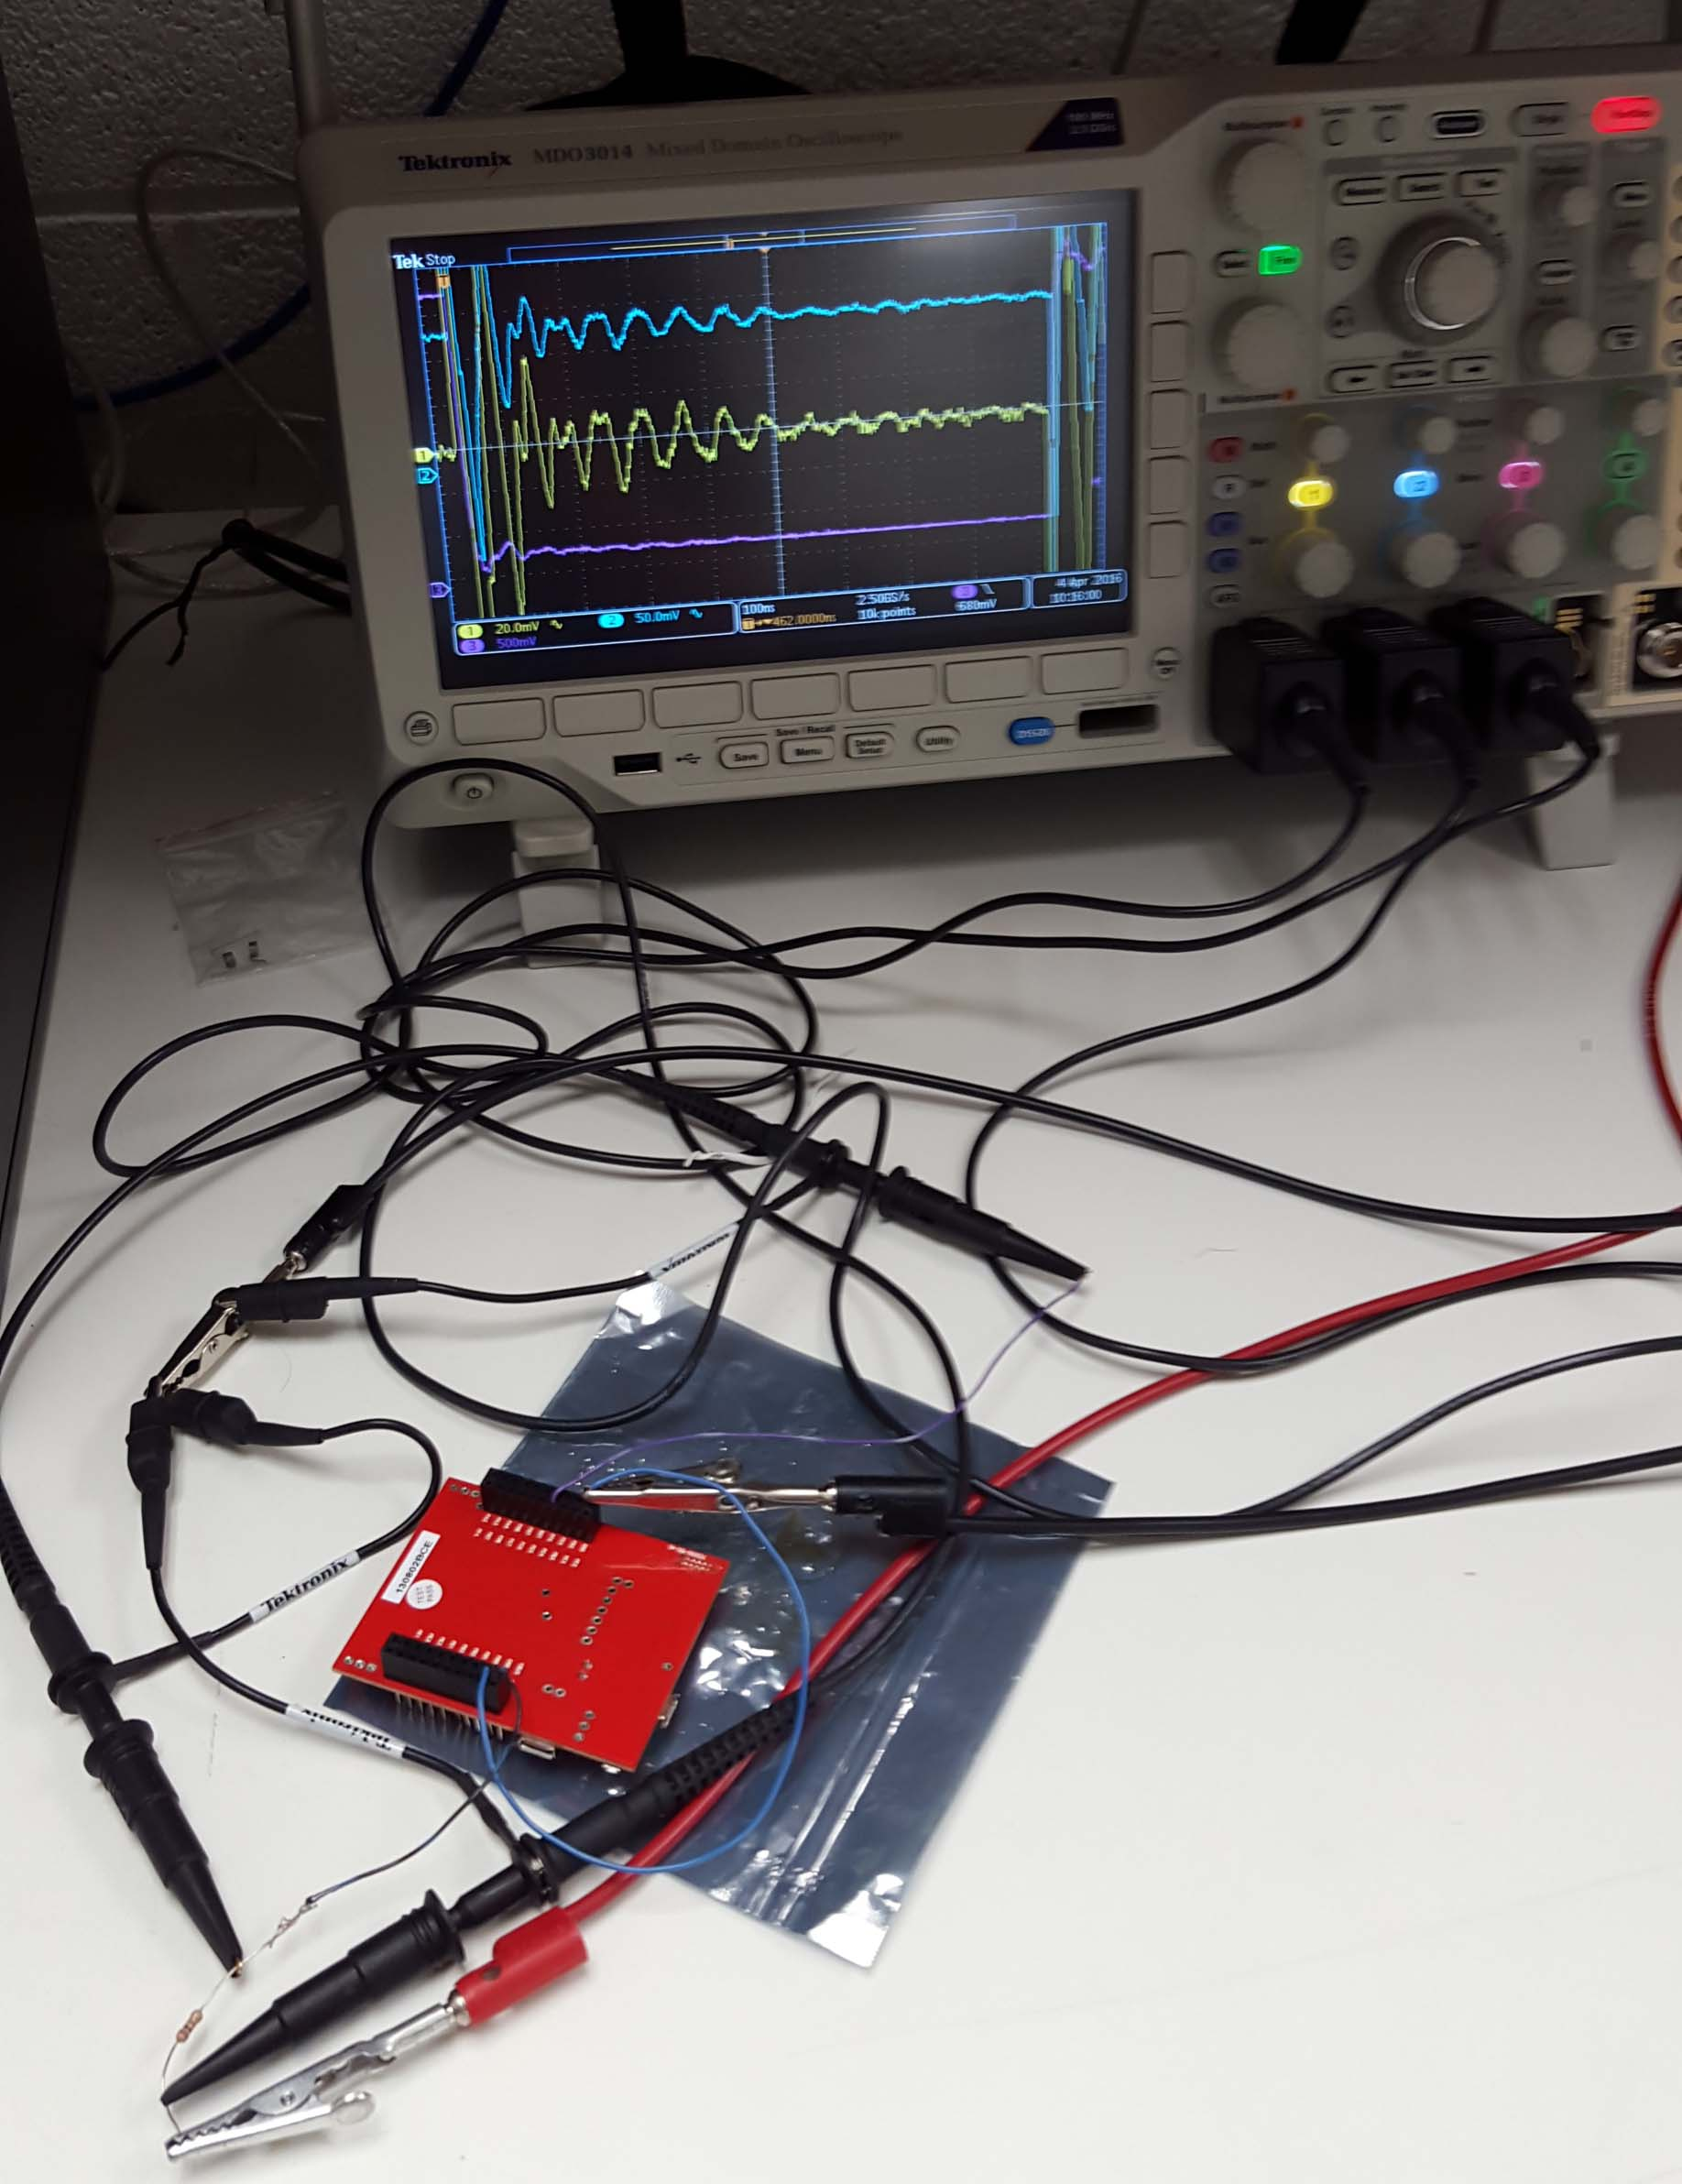
\includegraphics[scale=.1]{setup}
    \caption{A picture taken of the experimental setup used.}
\end{figure} 

\section{POWER TRACE ANALYSIS}


\section{RESULTS}
 
 %4bit 1: 677 0: 644

\section{CONCLUSION}

Some improvements for a future implementation of a DPA attack on a microcontroller running DES would be to use a better differential oscilloscope probe setup for power analysis. One of the channels was jumping around the viewing screen, which clipped some of the trace measurements during the recording process. Another improvement would be to get more traces during the record process. 4-bit DPA analysis should produce more accurate results than 1-bit DPA but using 4-bit DPA only results
in around 1,300 traces, while the 1-bt DPA uses about 10,000 traces. For the 4-bit DPA to be accurate, there would need to be at least an order of magnitude more traces sampled.


\addtolength{\textheight}{-12cm}   % This command serves to balance the column lengths
                                  % on the last page of the document manually. It shortens
                                  % the textheight of the last page by a suitable amount.
                                  % This command does not take effect until the next page
                                  % so it should come on the page before the last. Make
                                  % sure that you do not shorten the textheight too much.

%%%%%%%%%%%%%%%%%%%%%%%%%%%%%%%%%%%%%%%%%%%%%%%%%%%%%%%%%%%%%%%%%%%%%%%%%%%%%%%%



%%%%%%%%%%%%%%%%%%%%%%%%%%%%%%%%%%%%%%%%%%%%%%%%%%%%%%%%%%%%%%%%%%%%%%%%%%%%%%%%



%%%%%%%%%%%%%%%%%%%%%%%%%%%%%%%%%%%%%%%%%%%%%%%%%%%%%%%%%%%%%%%%%%%%%%%%%%%%%%%%

%\section*{ACKNOWLEDGMENT}

%The author would like to thank his instructor Dr. Rajnikant Sharma %for his help in understanding control concepts.




%%%%%%%%%%%%%%%%%%%%%%%%%%%%%%%%%%%%%%%%%%%%%%%%%%%%%%%%%%%%%%%%%%%%%%%%%%%%%%%%




\begin{thebibliography}{99}

\bibitem{c1} J. Orlin Grabbe. The DES Algorithm Illustrated. \emph{Laissez Faire City Times}, 2006.
\bibitem{c2} Thomas S. Messerges and Ezzy A. Dabbish, "Investigations of Power Analysis Attacks on Smartcards," \emph{USENIX Workshop on Smartcard Technology}, Chicago, Illinois, USA, 1999. 

\end{thebibliography}

\section{APPENDIX A}

\begin{center}
\begin{figure}[thpb]
	\centering
	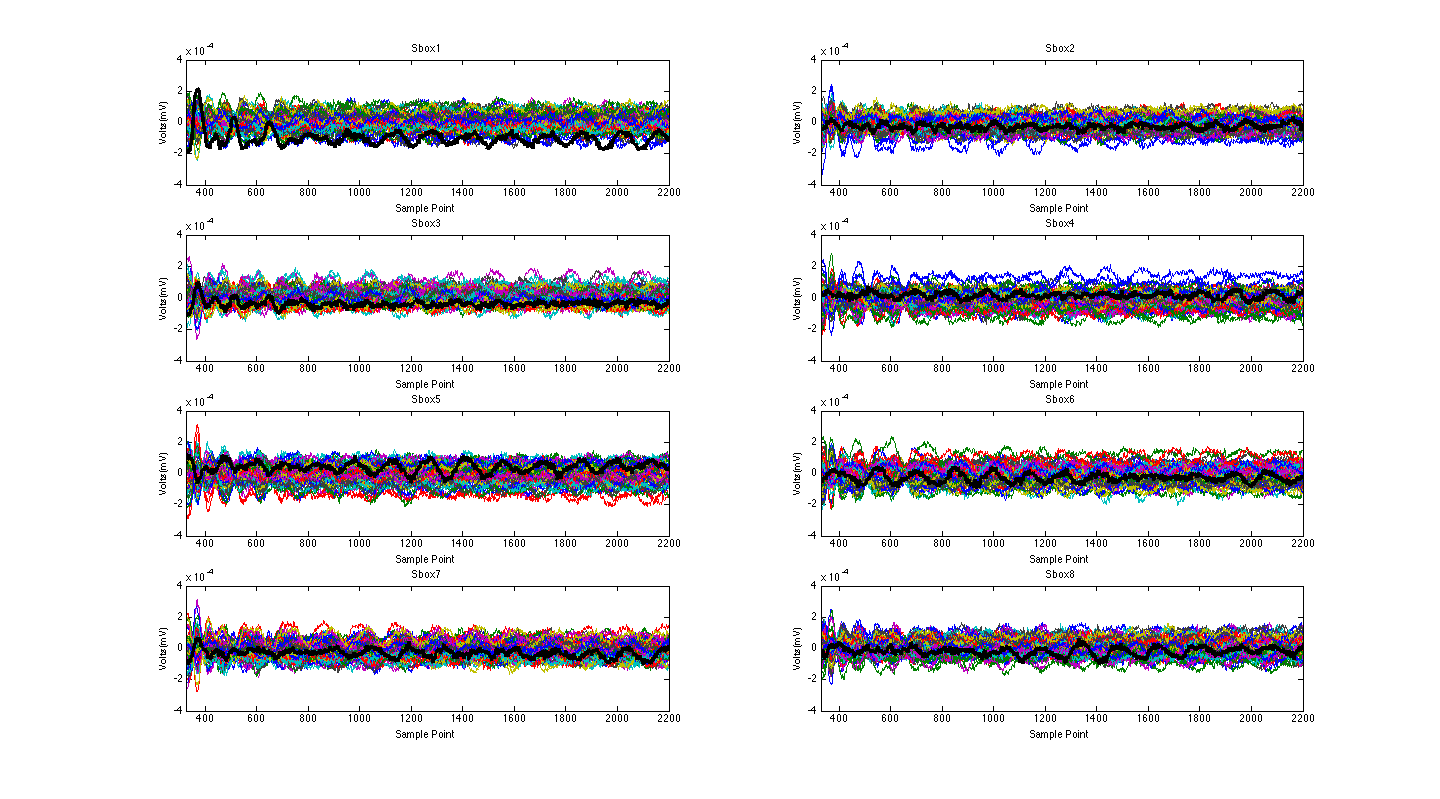
\includegraphics[scale=.45]{SBox_NormRes_1bit}
    \caption{Sbox power trace for 1 bit DPA using normal resolution.}
\end{figure}
\end{center}

\pagebreak

\begin{center}
\begin{figure}[thpb]
	\centering
	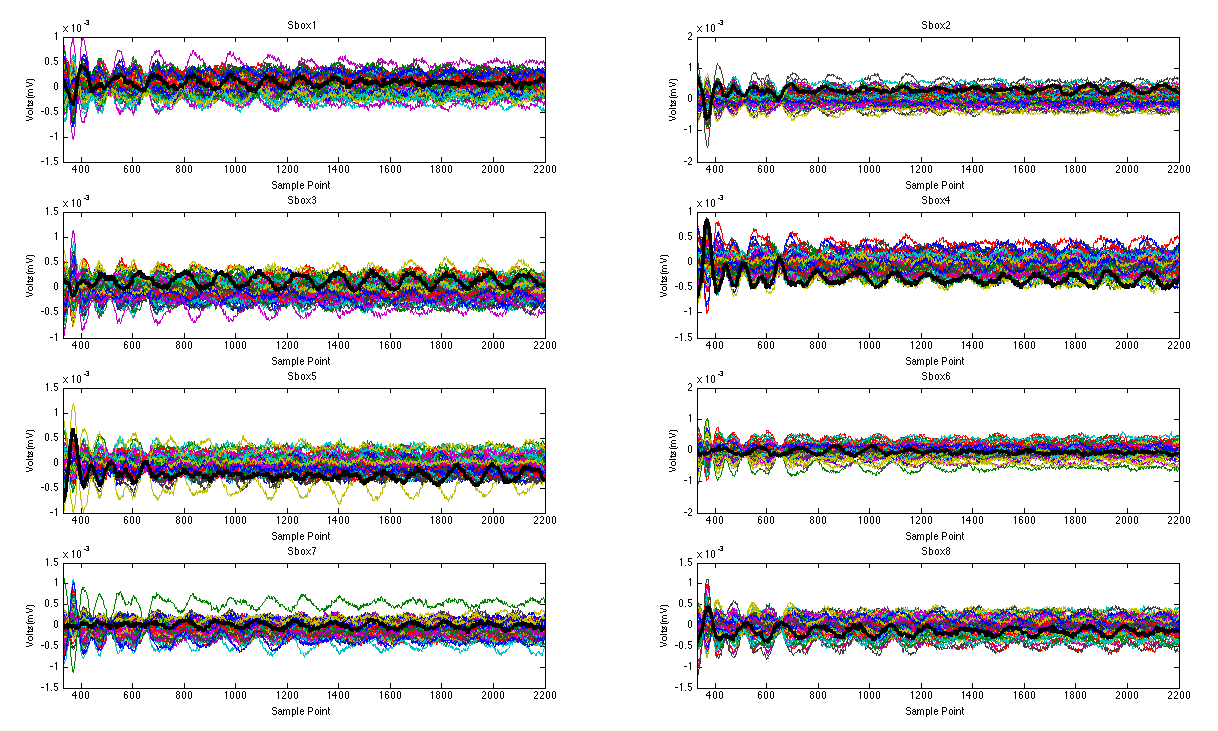
\includegraphics[scale=.45]{SBox_NormRes_4bit}
    \caption{Sbox power trace for 4 bit DPA using normal resolution.}
\end{figure}
\end{center}

\pagebreak

\begin{center}
\begin{figure}[thpb]
	\centering
	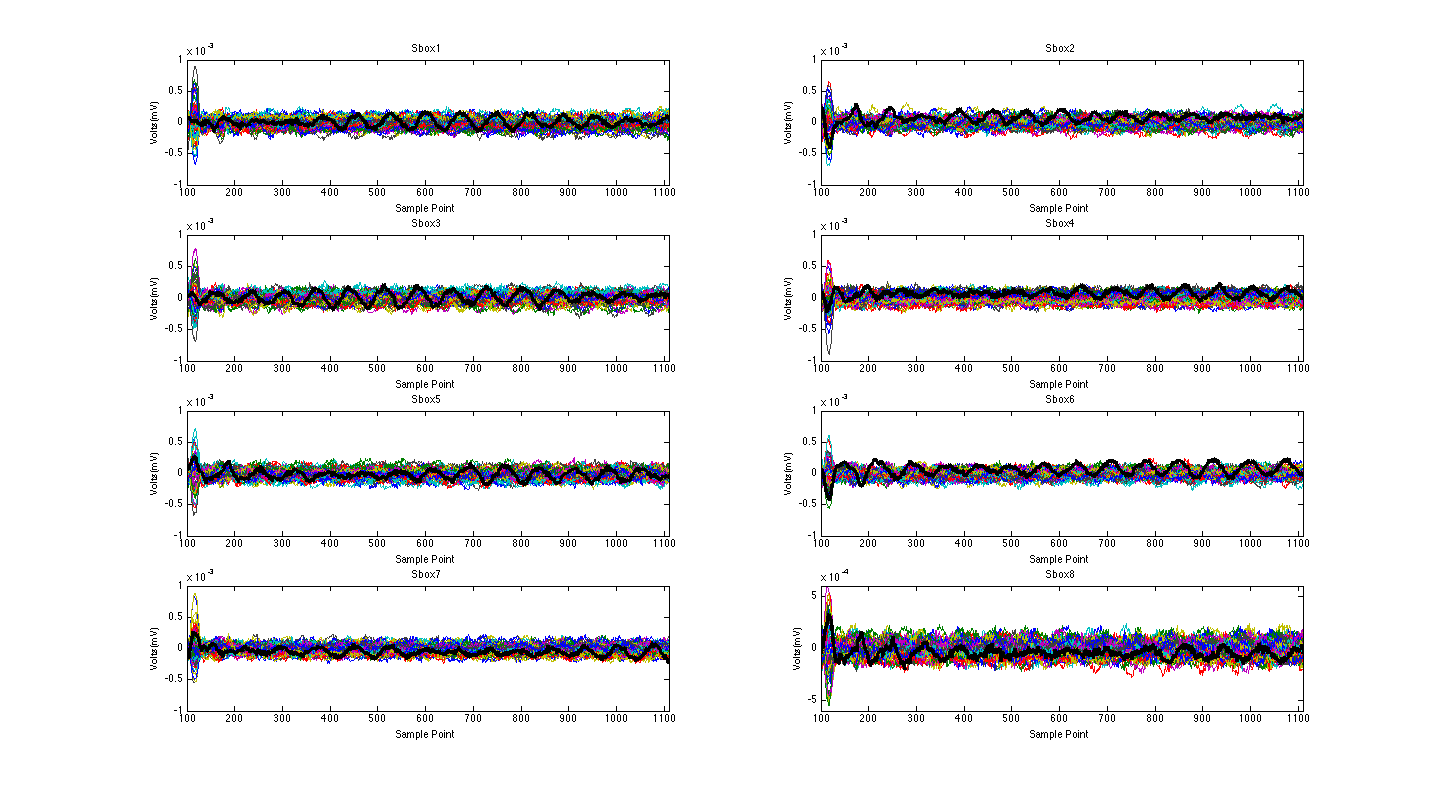
\includegraphics[scale=.45]{SBox_HiRes_1bit}
    \caption{Sbox power trace for 1 bit DPA using higher resolution.}
\end{figure}
\end{center}

\pagebreak

\begin{center}
\begin{figure}[thpb]
	\centering
	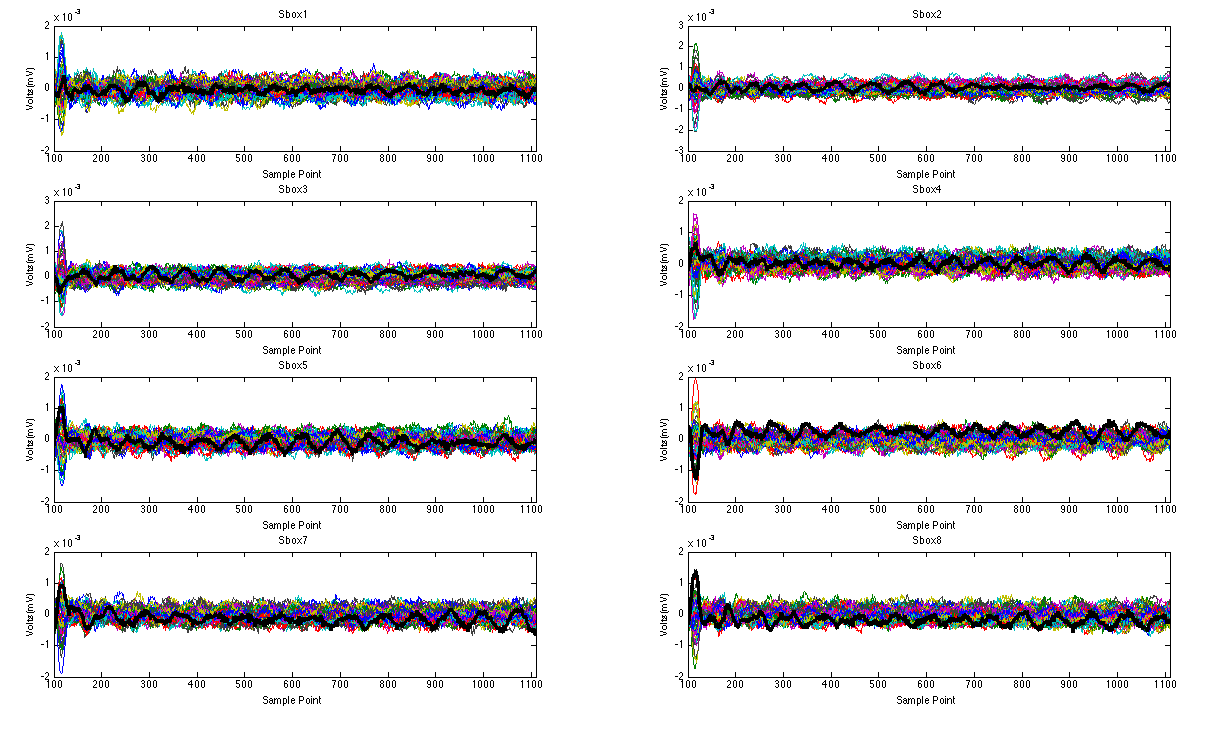
\includegraphics[scale=.45]{SBox_HiRes_4bit}
    \caption{Sbox power trace for 4 bit DPA using higher resolution.}
\end{figure}
\end{center}

\end{document}
